%%%
\subsection{Algorithm-Level Methods for Imbalanced Data}



%%%
\subsubsection{Bagging}

``Bagging'' is short for Bootstrapped Aggregating, a variation on random undersampling \citep{BRIEMAN_1996}.  In general, bagging takes many random subsets (with replacement) of the samples, run the classifier on each subset, then aggregate the results.  In imbalanced data applications, each subset of the samples is all of the $n$ minority samples and $n$ randomly chosen majority samples.  

Balanced Random Forest [need citation] is a form of bagging.  

In our example, bagging would make a subset of the data with the three minority-class samples (\#7, 8, and 9), and three randomly chosen from the majority-class samples, run the classifier; repeat some number of times.  Use an ensemble classifier to merge the results.  

\begin{center}
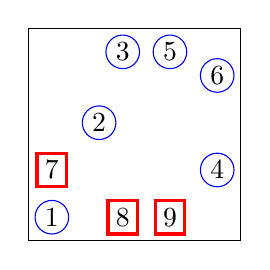
\begin{tikzpicture}[x = 3mm, y=3mm]
	\draw (-1,-1) rectangle (8,8);
	\tikzstyle{Square} = [
		draw = red, 
		very thick,
		rectangle,
		inner sep = 1mm,
		minimum size = 2 mm
	]
	\tikzstyle{SquareFill} = [
		draw = red, 
		fill = red,
		very thick,
		rectangle,
	]
	\tikzstyle{Circle} = [
		draw = blue, 
		circle,		
		inner sep = 0.5mm,
	]
	\tikzstyle{CircleFill} = [
		draw = blue,
		fill = blue, 
		circle,
	]
	\node [Circle] (1) at (0,0) {1};
	\node [Circle] (2) at (2,4) {2};
	\node [Circle] (3) at (3,7) {3};
	\node [Circle] (4) at (7,2) {4};
	\node [Circle] (5) at (5,7) {5};
	\node [Circle] (6) at (7,6) {6};
	\node [Square] (7) at (0,2) {7};
	\node [Square] (8) at (3,0) {8};
	\node [Square] (9) at (5,0) {9};

\end{tikzpicture}
\end{center}


%%%
\subsubsection{Boosting}

Boosting is an iterative method that runs the classifier multiple times.  At the end of each iteration, it determines which samples would be misclassified under the current model.  In the next iteration, the classifier gives higher weight to the misclassified samples, improving the model on marginal cases.  While boosting is not just for imbalanced data, the challenge in imbalanced data is that the minority class samples get misclassified, so boosting would help.  A popular implementation is AdaBoost, introduced by \cite{FREUND1997119}.
